\documentclass[12pt]{article}
%\renewcommand\normalsize{\fontsize{10pt}{12pt}\selectfont}
\usepackage{graphicx} % Required for inserting images
\usepackage[left=2cm,right=2cm,top=2cm,bottom=1.5cm]{geometry}

\title{Quiz 2}

\setlength{\parindent}{0pt}
\setlength{\parskip}{3mm}


\begin{document}

FS1 Wilkinson
Quiz 2, April 17 2025

1. The physics prof has attached a lacrosse ball to the end of a 1 meter string and is swinging it, making a pendulum. The ball's speed as it passes through the bottom of its arc is 2 m/s. 

a. Find the centripetal acceleration of the ball as it passes through the bottom of its arc.

\bigskip
\bigskip
\bigskip



b. The ball's mass is 0.1 kg. Calculate the tension in the string at the bottom of the arc. If you couldn't solve part (a), use $a=3$ m/s$^2$. (Hint: same process as finding the force Adam used to hang on to the swinging rope). You can approximate $g$ to be 10 m/s$^2$.

\bigskip
\bigskip
\bigskip
\bigskip
\bigskip
\bigskip

c. As the ball swings up and slows down, what happens to the tension in the string - less, the same, greater? Why? (Multiple reasons possible; one required for credit)

\bigskip
\bigskip
\bigskip
\bigskip


2. If there were a planet orbiting the sun in a circle at exactly 2 times Earth's orbit radius, how would its speed compare to Earth's? Justify your answer. Partial credit for correct conceptual answer, full credit for correct ratios of the speeds.

\bigskip
\bigskip
\bigskip
\bigskip
\bigskip


Bonus. The ball in problem 1 has centripetal acceleration at the bottom of the arc, where its $v$ is maximum. But on homework 1, when the pendulum bob had its maximum $v$, the slope of $v$ was zero and we said the acceleration was 0 - you can see it on the graph. What gives? 

 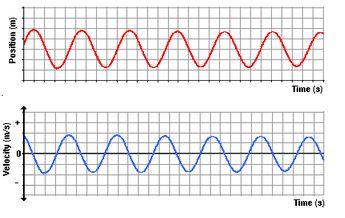
\includegraphics[width=0.4\linewidth]{C3.JPG}


\end{document}